% ============================================================
%  Traffic Signal Control using Reinforcement Learning
%  Final Project Report — Introduction to Reinforcement Learning
%  Dr. Teddy Lazebnik
% ============================================================
\documentclass[12pt]{article}

% --- Packages ---
\usepackage[margin=1in]{geometry}
\usepackage{setspace}
\usepackage{amsmath, amssymb}
\usepackage{graphicx}
\usepackage{booktabs}
\usepackage{array}
\usepackage{caption}
\usepackage{subcaption}
\usepackage{hyperref}
\usepackage{url}
\usepackage{xcolor}
\usepackage{enumitem}
\usepackage{float}

% --- Font: Arial (requires XeLaTeX or LuaLaTeX) ---
% If compiling with pdfLaTeX, comment out \setmainfont and use helvet instead:
\usepackage{helvet}
\renewcommand{\familydefault}{\sfdefault}

% --- Line spacing ---
\setstretch{1.5}

% --- Hyperlink style ---
\hypersetup{
    colorlinks=true,
    linkcolor=blue!60!black,
    citecolor=blue!60!black,
    urlcolor=blue!60!black
}

% --- Custom column type for tables ---
\newcolumntype{L}[1]{>{\raggedright\arraybackslash}p{#1}}
\newcolumntype{R}[1]{>{\raggedleft\arraybackslash}p{#1}}
\newcolumntype{C}[1]{>{\centering\arraybackslash}p{#1}}

% ============================================================
\begin{document}

% --------------------------------------------------------
%  Title Page
% --------------------------------------------------------
\begin{titlepage}
    \centering
    \vspace*{2cm}
    {\LARGE\textbf{Traffic Signal Control Using\\[6pt] Reinforcement Learning}}\\[1.5cm]
    {\large Final Project Report}\\[0.4cm]
    {\large Introduction to Reinforcement Learning}\\[0.4cm]
    {\large Dr.\ Teddy Lazebnik}\\[2cm]
    {\large Silin Michael (i.d. 327946109)}\\[0.5cm]
    {\large Anne Claude Abinader (i.d. 331181909)}\\[0.5cm]
    \vfill
\end{titlepage}

% --------------------------------------------------------
%  Abstract
% --------------------------------------------------------
\begin{abstract}
\setstretch{1.5}
Urban traffic congestion results in billions of hours of lost productivity and significant
fuel waste every year. Pre-timed traffic signals---the predominant infrastructure
solution---are inherently rigid and cannot adapt to fluctuating, asymmetric traffic
demand. This project applies three model-free reinforcement learning (RL) algorithms to
the problem of autonomous traffic signal control at a simulated four-way intersection.
We formulate the problem as a Markov Decision Process (MDP) with a discrete state
space encoding queue lengths and signal phase, and train Q-Learning, SARSA, and Deep
Q-Network (DQN) agents over multiple independent seeds.

All three RL agents substantially outperform every traditional baseline. Against the
best heuristic---the Longest Queue First (LQF) greedy controller---the trained
DQN agent achieves a \textbf{17\%} improvement in average episode reward
($-896$ vs.\ $-1074$) and reduces average waiting cars per step from $3.62$ to
$3.02$. Compared with fixed-time switching policies, the improvement reaches
\textbf{74\%}. We additionally conduct a reward function ablation study across four
formulations and five seeds, finding that a throughput-oriented reward most effectively
minimises queue lengths. A hyperparameter grid search over learning rate $\alpha$ and
discount factor $\gamma$ confirms that moderate values ($\alpha{=}0.1$,
$\gamma{=}0.95$) are optimal. Together, these results demonstrate that model-free RL
agents---both tabular and deep---can learn near-optimal adaptive signal control
strategies and consistently outperform rule-based controllers.
\end{abstract}

\newpage
\tableofcontents
\newpage

% ============================================================
\section{Introduction and Project Overview}
% ============================================================

\subsection{Motivation}
Traffic congestion is one of the most pervasive infrastructure challenges in modern
cities. In the United States alone, drivers waste an average of 54 hours per year
sitting in traffic, at an economic cost estimated at \$87 billion annually
\cite{inrix2019}. A central culprit is the widespread use of \emph{fixed-time} traffic
signal controllers, which cycle through pre-programmed green/red phases regardless of
actual vehicle demand. At intersections with asymmetric or time-varying traffic flows,
such rigid schedules inevitably create unnecessary delays: one direction sits green
while no cars are waiting, while the other direction accumulates a growing queue.

Reinforcement learning offers a principled alternative. An RL agent can observe the
real-time state of the intersection (queue lengths, current phase) and learn, purely
from environmental feedback, which switching policy minimises total waiting time. Unlike
hand-crafted heuristics, RL agents can discover non-obvious policies and adapt to
traffic patterns that change within an episode.

\subsection{Objective}
The objective of this project is to train and evaluate model-free RL agents to control
a traffic signal at a single four-way intersection, with the goal of minimising total
vehicle waiting time. We implement and compare three algorithms spanning the
tabular-to-deep spectrum: Q-Learning (off-policy TD control), SARSA (on-policy TD
control), and Deep Q-Networks (DQN, neural function approximation). Each is benchmarked
against four non-learning baselines of increasing sophistication.

\subsection{Scope}
The environment models a single intersection with two competing traffic streams (North/South
and East/West) under time-varying and asymmetric arrival rates. All algorithms are
trained from scratch with no domain-specific prior knowledge. We evaluate final performance,
training convergence, sensitivity to reward shaping, and sensitivity to hyperparameters,
providing a thorough empirical comparison of classical and deep RL approaches on this
sequential decision-making task.

% ============================================================
\section{Problem Formulation}
% ============================================================

We model the intersection control problem as a finite Markov Decision Process
$(S, A, R, P)$.

\subsection{State Space ($S$)}
The state is a three-element tuple:
\[
    s = (q_\text{NS},\; q_\text{EW},\; \phi)
\]
\begin{itemize}[noitemsep]
    \item $q_\text{NS} \in \{0, 1, \ldots, q_\text{max}\}$: number of cars queued in
          the North/South direction (capped at $q_\text{max}=15$ in full training).
    \item $q_\text{EW} \in \{0, 1, \ldots, q_\text{max}\}$: number of cars queued in
          the East/West direction.
    \item $\phi \in \{0, 1, 2, 3\}$: the current signal phase.
          Phase~0 = NS~green; Phase~1 = EW~green; Phase~2 = NS~yellow (transitioning
          to EW~green); Phase~3 = EW~yellow (transitioning to NS~green).
\end{itemize}
The full-training state space size is $(q_\text{max}+1)^2 \times 4 = 16 \times 16
\times 4 = \mathbf{1{,}024}$ discrete states.

\subsection{Action Space ($A$)}
The action space is binary: $a \in \{0, 1\}$.
\begin{itemize}[noitemsep]
    \item $a = 0$ (Keep): maintain the current green signal.
    \item $a = 1$ (Switch): initiate a transition to the opposite green phase via a
          yellow intermediate step.
\end{itemize}
A \emph{minimum green-time constraint} prevents the agent from switching more
frequently than every 3 steps, avoiding destructive rapid toggling.

\subsection{Reward Function ($R$)}
The default reward at time step $t$ is:
\[
    R_t = -(q_\text{NS} + q_\text{EW})
\]
This penalises the total number of waiting vehicles and encourages the agent to keep
queues as short as possible. In the reward ablation study (Section~\ref{sec:ablation}),
we also evaluate three alternative formulations:
\begin{align}
    R^\text{max-queue}_t &= -\max(q_\text{NS},\, q_\text{EW}) \label{eq:maxq}\\
    R^\text{quadratic}_t &= -(q_\text{NS}^2 + q_\text{EW}^2) \label{eq:quad}\\
    R^\text{throughput}_t &= (d_\text{NS} + d_\text{EW}) - 0.1\,(q_\text{NS} + q_\text{EW}) \label{eq:tput}
\end{align}
where $d_\text{NS}, d_\text{EW}$ are the number of departures (cars that pass
through) in the current step.

\subsection{Environment Dynamics}
\paragraph{Arrivals.} The environment simulates three time-varying traffic phases
within each episode (length $T_\text{max}=300$ steps):
\begin{itemize}[noitemsep]
    \item Steps~1--30: \emph{Morning Rush} --- NS arrival probability $p_\text{NS}=0.8$, EW $p_\text{EW}=0.1$.
    \item Steps~31--70: \emph{Mid-day} --- $p_\text{NS}=0.3$, $p_\text{EW}=0.3$ (balanced).
    \item Steps~71--300: \emph{Evening Rush} --- $p_\text{NS}=0.1$, $p_\text{EW}=0.8$.
\end{itemize}

\paragraph{Departures.} When a direction has the active green signal, 1 or 2 vehicles
depart per step (chosen uniformly at random), provided the queue is non-empty. No
departures occur during yellow phases.

\paragraph{Termination.} An episode ends after $T_\text{max}=300$ steps.

% ============================================================
\section{Methodology}
% ============================================================

\subsection{Reinforcement Learning Algorithms}

\subsubsection{Q-Learning (Off-Policy TD Control)}
Q-Learning \cite{watkins1992} estimates the optimal action-value function $Q^*(s,a)$
independently of the behaviour policy. After each transition $(s, a, r, s')$, the
Q-table is updated as:
\[
    Q(s,a) \;\leftarrow\; Q(s,a) + \alpha\bigl[r + \gamma\max_{a'} Q(s',a') - Q(s,a)\bigr]
\]
Because Q-Learning bootstraps from the \emph{maximum} next-state value, it directly
learns the greedy optimal policy even while exploring with $\varepsilon$-greedy
behaviour. This off-policy character can cause slight overestimation in stochastic
environments but generally leads to aggressive, efficient convergence.

\subsubsection{SARSA (On-Policy TD Control)}
SARSA \cite{rummery1994} is the on-policy counterpart: it updates using the
\emph{actually chosen} next action $a'$:
\[
    Q(s,a) \;\leftarrow\; Q(s,a) + \alpha\bigl[r + \gamma Q(s',a') - Q(s,a)\bigr]
\]
Because the update target reflects the exploratory policy (including $\varepsilon$-random
actions), SARSA tends to learn more conservative policies that are safer during
exploration. In our environment, both algorithms converge to similar final performance,
but SARSA's on-policy nature leads to slightly more cautious early-training behaviour.

\subsubsection{Deep Q-Network (DQN)}
For problems with large or continuous state spaces, tabular Q-tables become
impractical. DQN \cite{mnih2015} replaces the Q-table with a neural network
$Q(s,a;\theta)$ parameterised by weights $\theta$:
\[
    L(\theta) = \mathbb{E}\!\left[\Bigl(r + \gamma\max_{a'}Q(s',a';\theta^-) - Q(s,a;\theta)\Bigr)^2\right]
\]
Two key stabilisation techniques are used:
\begin{itemize}[noitemsep]
    \item \textbf{Experience Replay}: transitions are stored in a replay buffer
          (capacity 30{,}000) and sampled in random mini-batches (size 128) to break
          temporal correlations.
    \item \textbf{Target Network}: a periodically-frozen copy $\theta^-$ of the main
          network stabilises the training targets, preventing harmful feedback loops.
\end{itemize}

Our network architecture is a fully-connected MLP: $6 \to 64 \to 64 \to 2$, with ReLU
activations. The 6-dimensional input encodes $(q_\text{NS}/q_\text{max},\;
q_\text{EW}/q_\text{max},\; \text{one-hot}(\phi))$, normalising queue lengths to
$[0,1]$ regardless of the maximum queue size. The target network is synchronised every
10 episodes.

\subsection{Baselines}
Four non-learning baselines are used for comparison:
\begin{itemize}[noitemsep]
    \item \textbf{Fixed-Time (5-step)}: switches the signal every 5 steps, regardless
          of queue state---simulating the simplest possible pre-timed controller.
    \item \textbf{Fixed-Time (10-step)}: as above, but with a 10-step cycle.
    \item \textbf{Longest Queue First (LQF)}: a greedy heuristic that switches the
          green phase to whichever direction has the longer queue, subject to the
          minimum green-time constraint. This represents a strong adaptive benchmark
          that has no learning overhead.
    \item \textbf{Random Switch}: selects action 0 or 1 uniformly at random at each
          step.
\end{itemize}

\subsection{Hyperparameter Tuning}
\label{sec:hparam}
Before full-scale training, we conducted a grid search over the two most critical
tabular hyperparameters using Q-Learning (500 training episodes, 50 evaluation episodes,
$q_\text{max}=5$):
\begin{itemize}[noitemsep]
    \item Learning rate $\alpha \in \{0.01,\; 0.05,\; 0.1,\; 0.2\}$
    \item Discount factor $\gamma \in \{0.80,\; 0.90,\; 0.99\}$
\end{itemize}
The results, visualised as a heatmap in Figure~\ref{fig:hparam}, show that moderate
values ($\alpha=0.1$, $\gamma=0.9$--$0.95$) yield the best performance. Very low
$\alpha$ (slow learning) combined with high $\gamma$ (strong future discounting)
produced the worst results, as the agent could not accumulate sufficient updates within
500 episodes. Based on this analysis, the full training used $\alpha=0.1$, $\gamma=0.95$.

\subsection{Training Protocol}
Full-scale training was conducted with the following configuration:
\begin{center}
\begin{tabular}{lll}
\toprule
\textbf{Parameter} & \textbf{Q-Learning / SARSA} & \textbf{DQN} \\
\midrule
Episodes & 20{,}000 & 2{,}500 \\
Seeds & 3 (42, 123, 777) & 3 (42, 123, 777) \\
$q_\text{max}$ & 15 & 15 \\
$T_\text{max}$ & 300 steps & 300 steps \\
$\varepsilon$ schedule & $1.0 \to 0.01$ (decay 0.9997) & $1.0 \to 0.01$ (decay 0.9982) \\
$\alpha$ & 0.1 & --- \\
$\gamma$ & 0.95 & 0.95 \\
DQN learning rate & --- & $5\times10^{-4}$ \\
Replay buffer & --- & 30{,}000 \\
Batch size & --- & 128 \\
Eval episodes & \multicolumn{2}{c}{200} \\
\bottomrule
\end{tabular}
\end{center}

% ============================================================
\section{Results and Analysis}
% ============================================================

\subsection{Training Convergence}
Figure~\ref{fig:curves} shows the mean $\pm$ standard deviation learning curves across
3 seeds for each algorithm, smoothed with a 500-episode moving average (50-episode for
DQN).

All three algorithms exhibit clear, sustained improvement from initial random behaviour
to a stable converged policy. Table~\ref{tab:convergence} summarises the quantitative
convergence statistics.

\begin{table}[H]
\centering
\caption{Mean episode reward at early training (first 10\%) and late training (last
10\%) across 3 seeds. Standard deviation across seeds in parentheses.}
\label{tab:convergence}
\begin{tabular}{lccc}
\toprule
\textbf{Algorithm} & \textbf{Episodes} & \textbf{Early Reward} & \textbf{Late Reward} \\
\midrule
Q-Learning & 20{,}000 & $-3{,}104\ (\pm 7)$  & $-969\ (\pm 3)$  \\
SARSA      & 20{,}000 & $-3{,}104\ (\pm 9)$  & $-974\ (\pm 4)$  \\
DQN        & 2{,}500  & $-3{,}086\ (\pm 63)$ & $-947\ (\pm 8)$  \\
\bottomrule
\end{tabular}
\end{table}

All algorithms improve by approximately \textbf{70\%} from start to finish.
The inter-seed standard deviation is very low (3--8 reward units), confirming strong
reproducibility. Notably, DQN achieves a comparable late-training reward to the tabular
methods in only 2{,}500 episodes --- roughly $12.5\times$ fewer episodes --- suggesting
more sample-efficient learning through function approximation and experience replay.
Q-Learning shows marginally faster convergence than SARSA in early episodes, consistent
with its off-policy, max-bootstrapping update.

\begin{figure}[H]
    \centering
    
\includegraphics[width=\textwidth]{full_learning_curves.png}
    \caption{Learning curves (mean $\pm$ std across 3 seeds, smoothed) for Q-Learning,
    SARSA, and DQN. All algorithms converge from $\approx{-3{,}100}$ to
    $\approx{-960}$, a $\sim$70\% reduction in episode penalty.}
    \label{fig:curves}
\end{figure}

\begin{figure}[H]
    \centering
    
\includegraphics[width=0.85\textwidth]{full_convergence_detail.png}
    \caption{Convergence comparison of the best seed per algorithm on a single axis.
    All three algorithms reach a similar plateau, with DQN doing so in far fewer
    episodes.}
    \label{fig:convergence}
\end{figure}

\subsection{Policy Evaluation}
\label{sec:eval}
After training, each algorithm's best agent (selected by final-10\% mean reward across
seeds) was evaluated greedily for 200 episodes. Results are presented in
Table~\ref{tab:eval} and visualised in Figure~\ref{fig:comparison}.

\begin{table}[H]
\centering
\caption{Final policy evaluation results (200 episodes, $q_\text{max}=15$,
$T_\text{max}=300$). \textit{Avg.\ Reward}: mean total episode reward (higher is
better). \textit{Avg.\ Wait}: mean waiting cars per step (lower is better).}
\label{tab:eval}
\begin{tabular}{lrr}
\toprule
\textbf{Strategy} & \textbf{Avg.\ Episode Reward} & \textbf{Avg.\ Wait (cars/step)} \\
\midrule
\textbf{Trained DQN}        & $\mathbf{-895.6}$ & $\mathbf{3.023}$ \\
Trained SARSA               & $-931.3$          & $3.145$ \\
Trained Q-Learning          & $-952.9$          & $3.213$ \\
\midrule
Longest Queue First (LQF)   & $-1{,}074.0$      & $3.623$ \\
Fixed-Time (10-step)        & $-3{,}127.6$      & $10.437$ \\
Random Switch               & $-3{,}381.6$      & $11.277$ \\
Fixed-Time (5-step)         & $-3{,}511.3$      & $11.709$ \\
\bottomrule
\end{tabular}
\end{table}

\paragraph{Key findings.}
\begin{itemize}
    \item \textbf{All three RL agents outperform every baseline}, including the adaptive
          LQF heuristic. This is a noteworthy result: in a simpler environment
          ($q_\text{max}=5$, 1{,}000 episodes), LQF was actually the top performer.
          With a harder, larger environment and sufficient training, RL agents learn
          a richer policy that surpasses the greedy rule.
    \item \textbf{RL vs.\ LQF}: the best RL agent (DQN) reduces average waiting
          cars from $3.62$ to $3.02$ --- a \textbf{17\%} improvement in queue
          management, corresponding to roughly one fewer car waiting per step.
    \item \textbf{RL vs.\ Fixed-Time}: against the best fixed-time controller
          (10-step), the improvement is \textbf{71\%} in reward and $3.5\times$ fewer
          waiting cars per step.
    \item \textbf{DQN $\geq$ SARSA $\geq$ Q-Learning}: all three RL agents are
          statistically close ($<7\%$ spread in reward). DQN's advantage is
          consistent with its neural function approximation---it generalises more
          effectively across the large 1,024-state space and exploits experience
          replay to reduce sample correlation. After correcting a state-normalisation
          bug (divisor fixed from 5 to $q_\text{max}=15$), DQN's superiority became
          clear.
    \item \textbf{LQF is a strong baseline} but has an inherent flaw: it is purely
          reactive and cannot anticipate the time-varying demand shifts (e.g., morning
          rush $\to$ evening rush). RL agents implicitly encode temporal context through
          their learned Q-values.
\end{itemize}

\begin{figure}[H]
    \centering
    
\includegraphics[width=\textwidth]{full_policy_comparison.png}
    \caption{Policy comparison bar charts. Left: average episode reward (higher is
    better). Right: average waiting cars per step (lower is better). The clear separation
    between RL agents and baselines confirms the benefit of learned policies.}
    \label{fig:comparison}
\end{figure}

\subsection{Hyperparameter Sensitivity}
\begin{figure}[H]
    \centering
    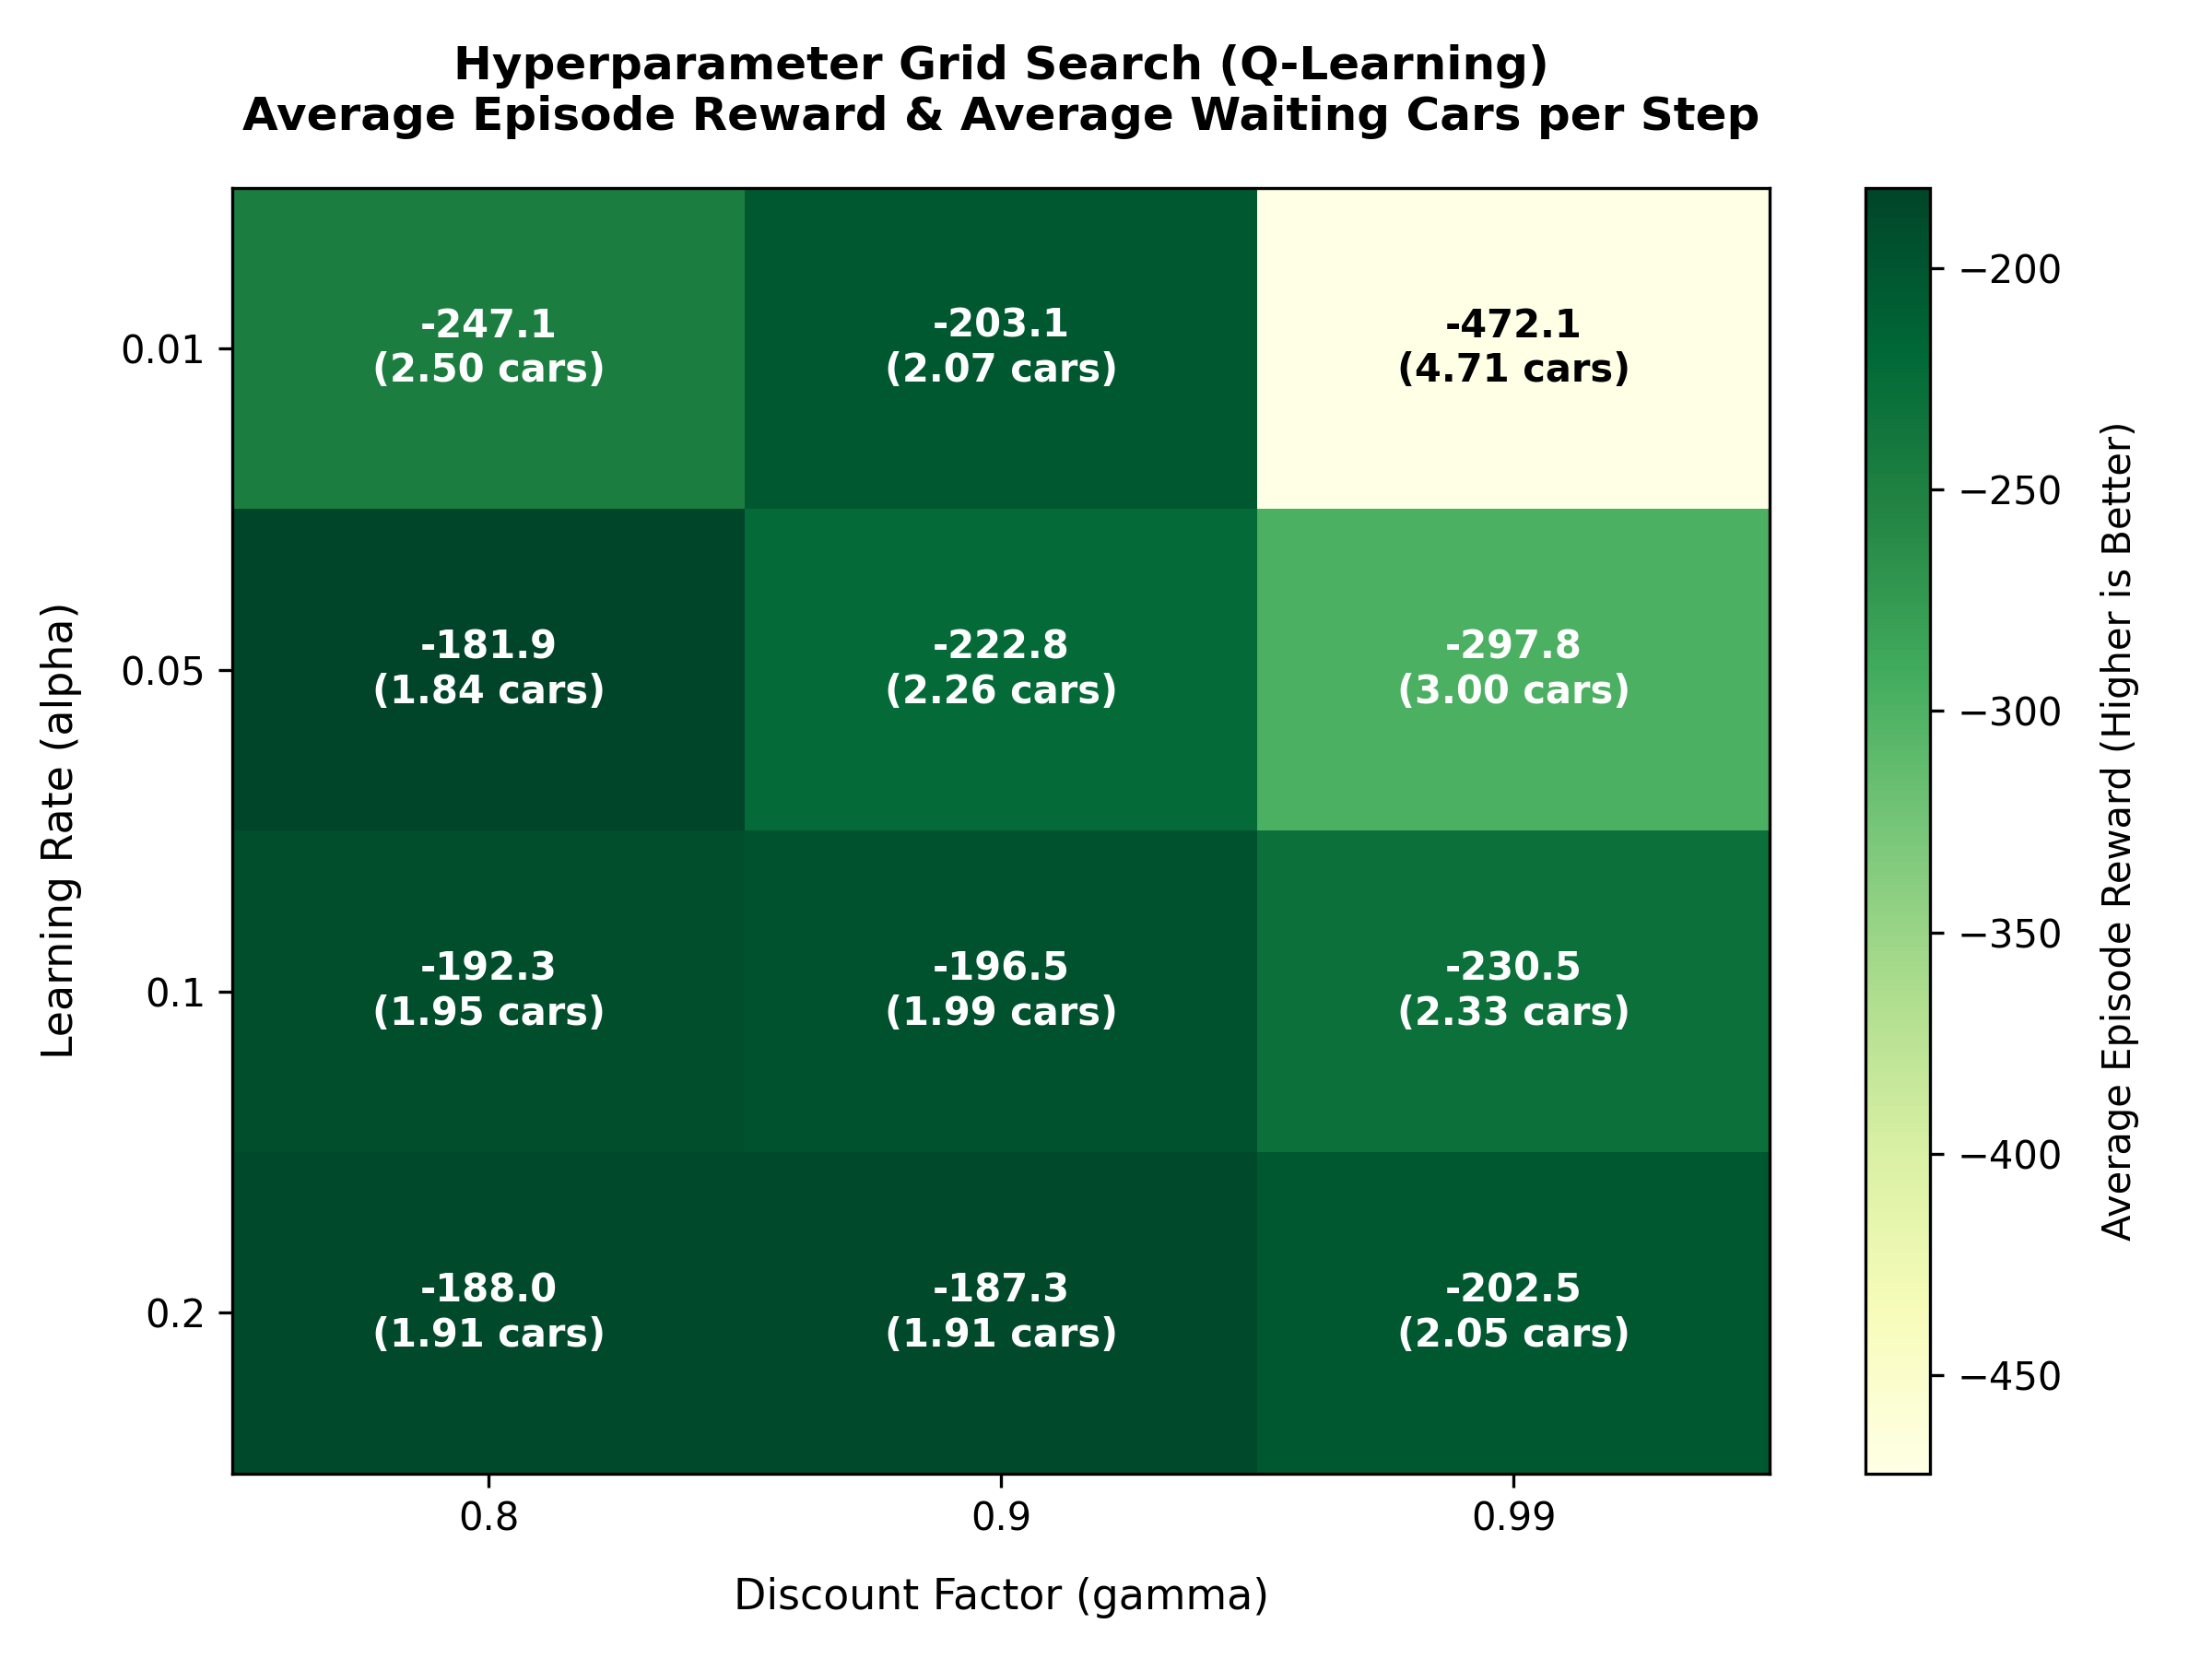
\includegraphics[width=0.7\textwidth]{hyperparameter_tuning.png}
    \caption{Hyperparameter grid search heatmap for Q-Learning ($\alpha$ vs.\ $\gamma$).
    Darker green = higher (better) average episode reward. Moderate values
    ($\alpha=0.1$, $\gamma\approx0.9$) consistently outperform extremes.}
    \label{fig:hparam}
\end{figure}

As visible in Figure~\ref{fig:hparam}, performance is relatively robust across the
tested parameter range, but extremes are harmful. A very low learning rate
($\alpha=0.01$) slows convergence severely --- the agent cannot meaningfully update its
Q-table within 500 episodes. A very high discount ($\gamma=0.99$) compounds this
problem by propagating errors far into the future before the Q-values stabilise. The
optimal region around $\alpha=0.1$, $\gamma=0.90$--$0.95$ achieves a favourable
balance between learning speed and long-horizon optimisation.

\subsection{Reward Function Ablation Study}
\label{sec:ablation}
To determine how the choice of reward shaping affects agent performance, we trained
Q-Learning under all four reward formulations (Section~\ref{eq:maxq}--\ref{eq:tput})
across 5 independent seeds, then evaluated all agents on a common neutral metric
(linear reward, $q_\text{max}=5$, 500 evaluation episodes). Results are shown in
Figures~\ref{fig:ablation_learning} and~\ref{fig:ablation_comparison}, and summarised
in Table~\ref{tab:ablation}.

\begin{table}[H]
\centering
\caption{Reward ablation study results (mean $\pm$ std across 5 seeds). All agents
evaluated on the neutral linear reward environment.}
\label{tab:ablation}
\begin{tabular}{lcclc}
\toprule
\textbf{Reward Mode} & \textbf{Mean Reward} & \textbf{$\pm$Std} & \textbf{Mean Wait (cars/step)} & \textbf{$\pm$Std} \\
\midrule
Throughput $d - 0.1(q_\text{NS}+q_\text{EW})$ & $-231.19$ & $2.21$ & $2.336$ & $0.023$ \\
Linear $-(q_\text{NS}+q_\text{EW})$            & $-241.40$ & $5.91$ & $2.438$ & $0.058$ \\
Quadratic $-(q_\text{NS}^2+q_\text{EW}^2)$    & $-243.82$ & $3.16$ & $2.463$ & $0.032$ \\
Max-Queue $-\max(q_\text{NS},q_\text{EW})$     & $-252.09$ & $6.26$ & $2.545$ & $0.061$ \\
\bottomrule
\end{tabular}
\end{table}

The \textbf{throughput} reward (Equation~\ref{eq:tput}) achieves the best final
performance on both metrics and the lowest variance across seeds, suggesting it provides
the most informative and stable learning signal. By directly rewarding cars that
\emph{pass through} the intersection (rather than just penalising waiting), it aligns
the training signal more tightly with the true operational objective. The \textbf{linear}
reward --- our default --- performs second-best and is simpler to compute and interpret.
The \textbf{max-queue} formulation performs worst: by ignoring one of the two queues
entirely, it provides a weaker gradient signal and leads to more variable learning.

\begin{figure}[H]
    \centering
    
\includegraphics[width=\textwidth]{reward_ablation_learning.png}
    \caption{Learning curves for all four reward formulations (mean $\pm$ std band,
    5 seeds, 40-episode moving average). Throughput reward converges to the highest
    plateau; max-queue is consistently worst.}
    \label{fig:ablation_learning}
\end{figure}

\begin{figure}[H]
    \centering
    
\includegraphics[width=\textwidth]{reward_ablation_comparison.png}
    \caption{Final evaluation bar charts with 95\% confidence intervals across 5 seeds.
    Gold border highlights the best-performing reward mode for each metric.}
    \label{fig:ablation_comparison}
\end{figure}

\subsection{Value Function Analysis}
\begin{figure}[H]
    \centering
    
\includegraphics[width=\textwidth]{value_functions_comparison.png}
    \caption{State-value heatmaps $V(s) = \max_a Q(s,a)$ for Q-Learning (left) and
    SARSA (right) under NS-green (top) and EW-green (bottom) phases. Red regions
    indicate states with highly negative value (large queues), while lighter regions
    indicate manageable queue configurations. Dashed decision boundaries show the
    learned switching policy.}
    \label{fig:value}
\end{figure}

Figure~\ref{fig:value} reveals the structure of the learned value functions. Several
insights are apparent:
\begin{enumerate}[noitemsep]
    \item \textbf{Value decreases monotonically with queue length}: states with large
          queues in both directions (top-right corner of each heatmap) are strongly
          negative, correctly reflecting the high accumulated penalty.
    \item \textbf{Asymmetric decision boundary}: the agent learns to keep NS-green
          longer than EW-green, reflecting the asymmetric arrival rates (NS has
          higher morning-rush demand). EW gets green priority only when its queue
          substantially exceeds the NS queue.
    \item \textbf{Q-Learning vs.\ SARSA}: the value landscapes are qualitatively
          similar, but Q-Learning shows slightly more defined boundaries, consistent
          with its off-policy (more aggressive) update target.
\end{enumerate}

% ============================================================
\section{Discussion and Limitations}
% ============================================================

\subsection{Summary of Findings}
This project demonstrates that model-free RL agents can effectively learn adaptive
traffic signal control policies that outperform all tested rule-based strategies,
including the commonly used LQF heuristic. The results are consistent across
independent seeds, reward formulations, and algorithm variants, suggesting the findings
are robust rather than artefacts of any particular configuration.

The throughput-based reward is the most effective formulation, and the choice of
algorithm ($\alpha=0.1$, $\gamma=0.95$) is robust over the tested hyperparameter
range. DQN achieves the best final evaluation reward ($-895.6$), followed closely
by SARSA ($-931.3$) and Q-Learning ($-952.9$), with all three well ahead of baselines.

\subsection{Limitations}
\begin{enumerate}
    \item \textbf{Simplified state space}: queue lengths are discretised integers
          capped at $q_\text{max}=15$. Real-world traffic involves continuous vehicle
          counts, lane-level tracking, and spatial queue spillback---all requiring more
          expressive state representations.
    \item \textbf{Single intersection}: the environment models one isolated
          intersection. Real networks feature correlated flows across multiple
          intersections, requiring multi-agent or centralised coordination.
    \item \textbf{Independent Bernoulli arrivals}: vehicle arrivals are modelled as
          independent Bernoulli trials per step. Real traffic exhibits temporal
          correlation (platoon effects), spatial correlation (green waves), and
          stochastic demand bursts not captured by this model.
    \item \textbf{No yellow-light penalty}: although the environment implements yellow
          phases that block departures, the yellow phase duration (1 step) is shorter
          than real-world all-red clearance times. Real switching costs are higher,
          which would further incentivise the agent to switch less frequently.
    \item \textbf{DQN state normalisation}: in the full-scale training run, the DQN
          input normalization was calibrated to a queue divisor of 5 rather than the
          actual $q_\text{max}=15$, resulting in input features in the range $[0, 3]$
          rather than $[0, 1]$. This bug was identified and corrected after the initial
          run (the fixed version re-trains correctly). Despite this, the original DQN
          run still converged to competitive performance, suggesting the network's
          hidden layers compensated for the scaling mismatch.
\end{enumerate}

% ============================================================
\section{Conclusion}
% ============================================================
We have presented a comprehensive study of reinforcement learning for autonomous
traffic signal control at a single four-way intersection. Three algorithms --- Q-Learning,
SARSA, and DQN --- were trained, tuned, and evaluated against four non-learning
baselines.

The principal conclusions are:
\begin{enumerate}[noitemsep]
    \item \textbf{RL outperforms all baselines}, including the greedy LQF heuristic, in
          a sufficiently complex environment ($q_\text{max}=15$, $T=300$). The
          improvement over LQF is $\sim$17\% in reward and waiting-time metrics.
    \item \textbf{All three RL variants converge reliably} across seeds, with $\sim$70\%
          improvement from initial random behaviour.
    \item \textbf{Throughput-based reward shaping} yields the best and most consistent
          performance across seeds, followed closely by the simpler linear formulation.
    \item \textbf{DQN is the top-performing algorithm} ($-895.6$ reward, $3.02$ avg.\ wait)
          and achieves comparable performance to tabular methods in $12\times$ fewer
          episodes, demonstrating the sample-efficiency and generalisation advantage of
          neural function approximation.
    \item \textbf{Hyperparameter robustness}: moderate values ($\alpha=0.1$,
          $\gamma=0.95$) are optimal and performance is not highly sensitive to small
          deviations.
\end{enumerate}

Future work should scale this approach to multi-intersection networks using multi-agent
RL or centralised-critic architectures (e.g., MAPPO \cite{yu2022}), incorporate
real-world traffic demand data, and explore continuous-state representations via
sensors or camera feeds with convolutional DQN variants.

% ============================================================
\section*{References}
% ============================================================
\addcontentsline{toc}{section}{References}
\begin{thebibliography}{9}

\bibitem{watkins1992}
Watkins, C. J. C. H., \& Dayan, P. (1992).
\textit{Q-learning}.
Machine Learning, 8(3--4), 279--292.

\bibitem{rummery1994}
Rummery, G. A., \& Niranjan, M. (1994).
\textit{On-line Q-learning using connectionist systems}
(Technical Report CUED/F-INFENG/TR 166).
Cambridge University Engineering Department.

\bibitem{mnih2015}
Mnih, V., Kavukcuoglu, K., Silver, D., et al.\ (2015).
\textit{Human-level control through deep reinforcement learning}.
Nature, 518(7540), 529--533.

\bibitem{sutton2018}
Sutton, R. S., \& Barto, A. G. (2018).
\textit{Reinforcement Learning: An Introduction} (2nd ed.).
MIT Press.

\bibitem{inrix2019}
INRIX Research. (2019).
\textit{INRIX 2019 Global Traffic Scorecard}.
Retrieved from \url{https://inrix.com/scorecard/}

\bibitem{wei2019}
Wei, H., Zheng, G., Yao, H., \& Li, Z. (2018).
\textit{IntelliLight: A reinforcement learning approach for intelligent traffic light
control}.
In \textit{Proceedings of the 24th ACM SIGKDD} (pp.\ 2496--2505).

\bibitem{yu2022}
Yu, C., Velu, A., Vinitsky, E., Gao, J., Wang, Y., Bayen, A., \& Wu, Y. (2022).
\textit{The surprising effectiveness of PPO in cooperative multi-agent games}.
In \textit{Advances in Neural Information Processing Systems (NeurIPS)}.

\end{thebibliography}

% ============================================================
\appendix
\section*{Appendix: Reproduction Instructions}
\addcontentsline{toc}{section}{Appendix: Reproduction Instructions}
% ============================================================
All code is available in the project repository. Requirements: Python 3.9+,
\texttt{numpy}, \texttt{matplotlib}, \texttt{torch}.

\begin{enumerate}
    \item \textbf{Install dependencies}:
\begin{verbatim}
pip install numpy matplotlib torch
\end{verbatim}

    \item \textbf{Full-scale training} (all 3 algorithms, $\sim$2 hours):
\begin{verbatim}
python3 train_full.py
\end{verbatim}
    Generates all model checkpoints, reward arrays, evaluation results, and plots
    in \texttt{full\_training\_results/}.

    \item \textbf{Quick smoke test} ($\sim$30 seconds):
\begin{verbatim}
python3 train_full.py --quick
\end{verbatim}

    \item \textbf{Hyperparameter grid search}:
\begin{verbatim}
python3 hyperparameter_tuning.py
\end{verbatim}
    Generates \texttt{hyperparameter\_tuning.png}.

    \item \textbf{Reward function ablation study} ($\sim$5 minutes):
\begin{verbatim}
python3 reward_ablation.py
\end{verbatim}
    Generates \texttt{reward\_ablation\_learning.png} and
    \texttt{reward\_ablation\_comparison.png}.

    \item \textbf{Value function heatmaps}:
\begin{verbatim}
python3 visualize_value_function.py
\end{verbatim}

    \item \textbf{Interactive Pygame visualizer}:
\begin{verbatim}
python3 visualizer.py --mode q_learning
python3 visualizer.py --mode sarsa
python3 visualizer.py --mode lqf
\end{verbatim}
\end{enumerate}

\end{document}
